\chapter{Discussion}

\section{Waveform Morphology}
The results we got for the waveform morphologies did not speak entirely with the results that Weder et al. \citeyear{Weder2018} reported. In most of the cases, larger sound pressure level did result in greater positive change of oxygenated hemoglobin concentration, or in other words, greater negative change in deoxygenated hemoglobin concentration. However, the results were not consistent between participants. The separation between different sound pressure levels could not be clearly seen. Apart from the results with the loudest audio stimuli, responses from other quieter audio stimuli were rather indistinguishable. Moreover, regarding the type of responses we measured from different regions of the left brain hemisphere, phasic response could be observed from the channels over the supramarginal superior temporal gyrus from most of the participants. However, only from some of the paritcipants, channels over Broca's area could show a broad tonic pattern as Weder et al. \citeyear{Weder2018} described.

\section {Regional Analysis}
In comparison to the research from Weder et al. \citeyear{Weder2018}, we chose a different approach to define our region of interest. Instead of first looking at the results and grouping different regions according to similar waveforms, we were more interested to know how the responses from the auditory cortex would be compared with other regions of the measured left brain hemisphere, so we grouped the three channels over the caudal superior temporal gyrus as one region (ROI 2), and the rest of the channels as another region (ROI 1).

The auditory cortex ~\ref{fig:CerebralCortex} was our interest of this study. It is around the caudal superior temporal gyrus. We compared the hemoglobin response from the three channels over the auditory cortex with all the other channels lying on the rest of the measured left brain hemisphere. The waveform morphology of the auditory cortex is very similiar to the counterparts of the rest of the measured parts. In other words, the dynamic hemoglobin response of the auditory cortex represents that of the entire left brain hemisphere fairly well.

\begin{figure}[H]
  \centering
     \copyrightbox[b]{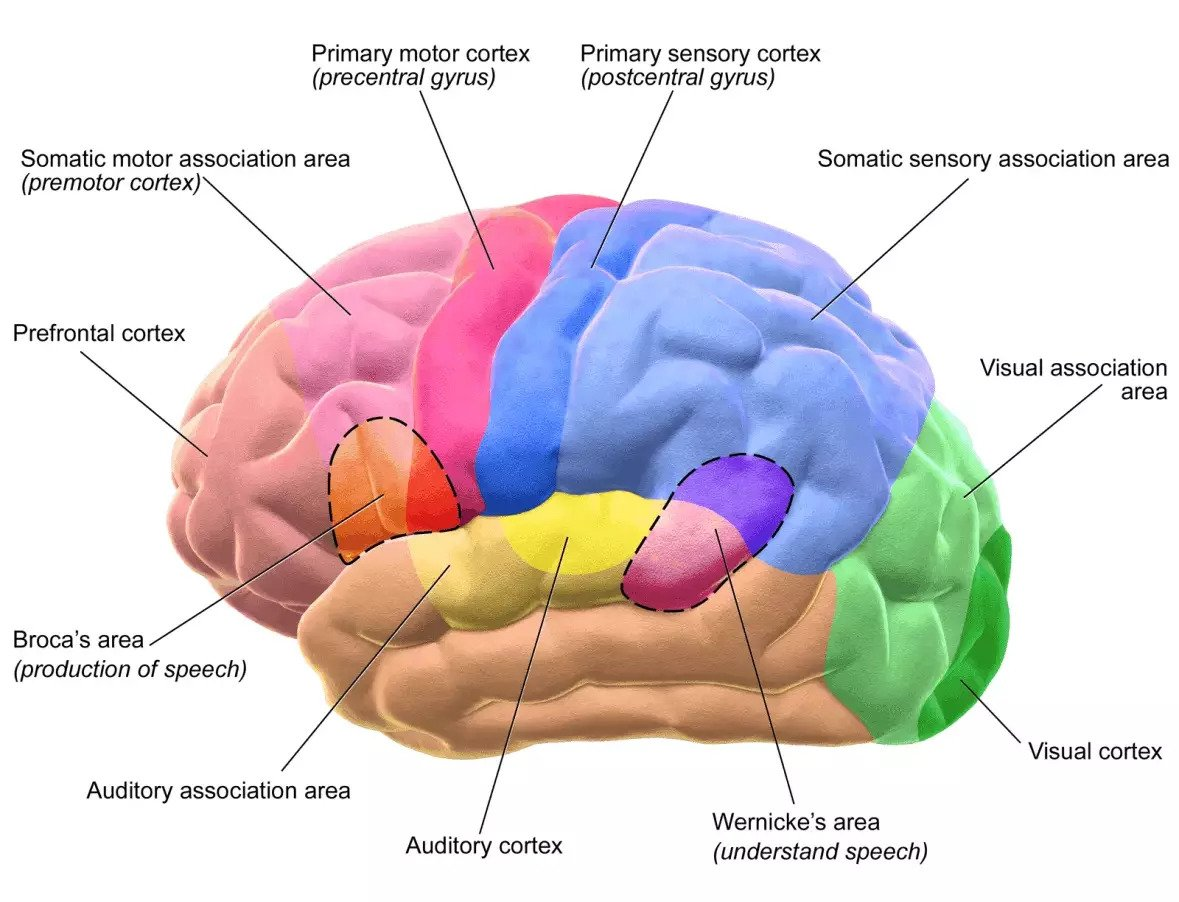
\includegraphics[scale=.3]{bilder/cerebral_cortex.jpg}}%
           {Source: \url{https://human-memory.net/sensory-cortex/}}
  \caption{Motor and Sensory Regions of the Cerebral Cortex}
  \label{fig:CerebralCortex}
\end{figure}

\section{Device Limitation and fNIRS Testing Conditions}

There could be several factors that potentially caused the results from this project to vary from that Weder et al. \citeyear{Weder2018} reported. First, we used the device Brite23. It is also a continuous-wave fNIRS device. The sources emitted light of slightly different wavelengths, which are 757 nm and 843 nm, whereas Weder et al. \citeyear{Weder2018} uses the device (NIRScout, NIRX, Germany) which sources emitted light of wavelengths 760 nm and 850 nm. Additionally as for the fNIRS testing procedure, we could have also improved on several things. To begin with, a darker sound booth would be more suitable. In our setup, the testing was also performed in a sound booth, but with normal light condition. Still, if the lighting was dimmer, there could be less noise in the hemoglobin response from visual stimulation. In addition, it would make sense to stabilize the participant's neck with a neck cushion. Not only would it be more comfortable for the participants during the measurement. Movement artifacts could also be reduced. Moreover, by including breaks in between can help participant maintain better attention.

Also, from our measurements, data from female participants with long hair had worse data quality. In our configuration, since we were only measuring the left brain hemisphere. First asking the participant to put the hair to the right side made it easier to put the cap on. Sometimes when the participants had thick long hair, trying to put the hair aside can be a futile attempt, but it was easier when they first put the hair to the other side. Last but not least, we would be curious to know how would the hemoglobin response from more people be like. If possible, more participants should be measured so the results from the project can be more credible. For example, participants of different ages and every gender and race would be desirable for this hearing research. Besides, other than only measure normal-hearing people, it would also be of our great interest to measure some cochlear implant users and compare the results together.

\section {Data Processing}
Our measured data was processed with a modified approach. In the research from Weder et al. \citeyear{Weder2018}, data pre-processing and analysis was executed in MATLAB and SPSS (version 24, IBM Corp., USA). They combined custom-made MATLAB scripts with Homer2 functions. On the other hand, the newer Homer3 with our MATLAB script in this study. Judging from the varying individual results, group analysis or statistical analysis will not be applicable in this case. Hence, the software program for statistical analysis, SPSS, was not used in this project. Furthermore, the differential pathlength factor (DPF) for each participant was calculated from their age. The resultant HbO and HbR concentration was estimated with the correction factor, whereas Weder et al. \citeyear{Weder2018} did not mention how they chose or calculated the DPF values.

\section{Loudness Perception}
In this project, results from individuals varied much. Although in hearing research, response from normal-hearing participants should be similar and reproducible, it is also well-know that, even between normal-hearing listeners,
considerable differences still exist in loudness perceptions \cite {Brand2001}. A more recent research \cite {Weder2020} was conducted in detail, and showed that Brain activation in response to different stimulus intensities is more reliant upon individual loudness sensation than the physical stimulus properties. Therefore, the authors suggested that loudness
estimates should be examined when interpreting results, especially when it comes to measurements using different auditory stimulus intensities. Different loudness perception can explain the varying results from individual participants.

\section{Audio Stimuli}
ICRA noises were chosen as the stimuli in this study because it is believed to be able to activate broad cortical auditory areas. However, some other researches were able to detect differences in cortical responses to speech of different intelligibility. Pollonini et al. \citeyear{Pollonini2013} found that normal speech evoked stronger repsonses within the auditory cortex than distorted speech did, and environmental sounds produced the least cortical activation. ICRA noises are amplitude-modulated noises, are completely unintelligible, and thus, belong to the distorted-speech category. Although ICRA noises may be able to activate broader cortical auditory areas than simple static stimulus, normal speech can perhaps produce even stronger responses within auditory cortex, according to Pollonini et al. \citeyear{Pollonini2013}. In addition, by providing intelligible normal speech as a stimuli rather than unintelligible noise, the measurement process can be less boring for the participants. They can then be more compliant and thus maintain better attention to actively listen to the soundtracks.

\section{Language Processing in Human Brains}
One primary goal of fNIRS researches is to improve a patient's ability to discriminate speech. In many researches, topics associated with hearing and language processing were investigated. However, language perception and processing in human brain do not have to be involved with audio stimuli. Visual-only speech can also activate language processing in the human brain. Shader et al. \citeyear{Shader2021} used both auditory-only and visual-only connected speech as stimuli in their research. Their results suggested that Heschl's gyrus may be the most advantageous location for identifying hemodynamic responses to complex auditory speech signals using fNIRS, for measuring responses to visual speech with fNIRS, regions corresponding to the facial processing pathway in occipital lobe can be more advantageous.

\section{Laterality of Brain Activation}
In this study, the fNIRS optodes were all placed on the left brain hemisphere, since according to Frost et al. \citeyear{Frost1999-vs}, language processing is strongly left lateralized. Nonetheless, from other papers, different results were observed and did not speak with the conclusion from Frost et al. \citeyear{Frost1999-vs}. For example, the data from Pollonini et al. \citeyear{Pollonini2013} is more reponsive to changes in activation within the right hemisphere. Belin et al. \citeyear{Belin2000} showed that the voice-selective regions can be found bilaterallly along the upper bank of \acrshort{sts}. Shader et al. \cite{Shader2021} also measured relatively symmetrical patterns across both hemispheres. Hence, if it is more advantageous to measure the left hemisphere for cortical response to audiometric stimuli with fNIRS remains till this point a question to be answered.

\section{Depth and Location of Cortical Response} % to Complex Auditory Speech Signals 
The depth of cortical response to complex auditory speech signals can also greatly affect the fNIRS measurements. Strangman et al. \citeyear{Strangman2013} demonstrated that sensitivity in depth decreases exponentially and diminishing returns appear to begin around 40 to 50 mm source-detector separations.

The left inferior frontal gyrus ~\ref{fig:gyrus}, or more specifically Broca's area ~\ref{fig:CerebralCortex} is implicated in higher-level linguistic processing \cite{Belin2000}. While in some studies \cite{Wijayasir2017} \cite{Zhou2018}, significant cortical activity in response to auditory speech signlas in this region can be detected, it was not always the case \cite{Musthtaq2019}. The studies that observed significant activation in the frontal region used fMRI or a combination of fMRI and fNIRS. It is possible that speech-evoked activity in the inferior frontal gyrus is isolated to the deeper cortical areas, so it's less likely to be detected with \acrshort{fnirs}. Different neuro-imagining methods can also explain why some studies \cite {Frost1999-vs} reported language processing to be left-laterialized whereas in other studies \cite{Shader2021}, opposite results were observed. It is possible that speech-evoked activities is related to the deeper cortical areas in the left hemisphere while the stimuli evoked responses in more superficial areas of the right cortex, making them more easily detected by fNIRS.

\begin{figure}[h]
  \centering
     \copyrightbox[b]{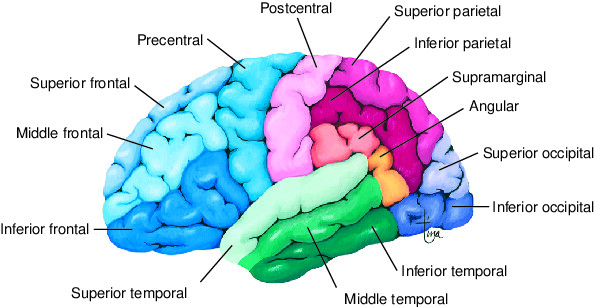
\includegraphics[scale=.5]{bilder/gyrus.jpeg}}%
           {Source: \url{https://www.tabers.com/tabersonline/view/Tabers-Dictionary/734639/all/gyrus}}
  \caption{Gyrus}
  \label{fig:gyrus}
\end{figure}


\section{HbR and HbO Data}
Most fNIRS studies only present HbO data \cite{Ferrari2012}, since it has a lower noise level, and thus more obvious responses can be observed. However, with our system, no significant difference was found regarding the HbO and HbR noise levels for most of the participants. Only some channels were measured with higher noise levels for the HbR data collected from participant 6. Unlike what Weder et al. \citeyear{Weder2018} presented in their paper, we were surprised to be able to measure comparably large HbO and HbR responses.


